%!TEX root = ../Master.tex
\section{Fokusområde} % (fold)

I forbindelse med kontekstanalysen for projektet, blev der foretaget et interview med kassereren i Vestre Baadelaug, Peter Hinrup, og sekretæren i Sejlklubben Limfjorden, Dorthe Carøe. Formålet med interviewet var at få et indblik i hvordan en sejlklub og dertilhørende havn er bygget op. Herunder hvilke administrationsopgaver der eksisterer, hvordan disse håndteres, og eventuelle problemstillinger herved. 

Interviewet blev foretaget i Vestre Baadelaugs klubhus, den 13. februar 2014, af Kasper Terndrup fra SW2-A405a og Martin Raunkjær Andersen fra SW2-A304, med Mikkel Madsen fra SW2-A405a som referent. Interviewet bestod af 3 dele. Den første del var en verbal fremlæggelse fra Peter Hinrup og Dorte Carøe omkring klubbernes generelle funktionalitet og interesser. Efterfølgende foretog Peter Hinrup en demonstration af Vestre Baadelaugs IT-system, Navision, med kommentarer angående systemet i forhold til klubbens behov. Til slut blev der stillet en række forberedte spørgsmål, som skulle sikre at alle ønskede emner blev dækket. Første og sidste del af interviewet blev optaget på lyd, og demonstrationen i anden del, blev filmet.

Interviewet resulterede i et generelt indblik i miljøet, der eksisterer i Vestre Baadehavn og Skudehavnen, samt miljøet blandt alle lystbådehavne i samarbejdet Aalborg-Nørresundby Fritidshavne (ANF). Derudover gav interviewet en god forståelse af Vestre Baadelaug som organisation med fokus på de administrative dele af bestyrelsen, samt en beskrivelse af demografien, som udgør medlemmerne.

Store dele af kontekstanalysen vil blive begrundet i udtalelser fra interviewet. Interviewet gav os indblik i Vestre Baadelaugs nuværende IT-system Navision. Systemet var velfungerende og dækkede deres behov. En beskrivelse af systemet følger nedenunder. 

\subsection{Nuværende IT-system} % (fold)
\label{sub:nuv_it_system}
Navision er et regnskabsprogram, i dag også kendt som Microsoft Dynamics NAV. Det blev oprindeligt udviklet af Jesper Balser, Torben Wind og Peter Bang tilbage i 1984. Siden da, har det haft forskellige navne. I 2002 opkøbte Microsoft programmet, og integrerede det i deres Microsoft Business Solutions program \cite{visiondata}.

Programmet samler en virksomheds aktiver i en grafisk brugerflade, der gør det enkelt at manipulere data som f.eks.\ medlemmer, materialer og økonomi. Navision er designet til at kunne håndtere alle typer virksomheder, og kan skræddersyes efter behov. Dette sker dog ved besøg af timelønnet programmør.

%\begin{figure}
%  \centering
%  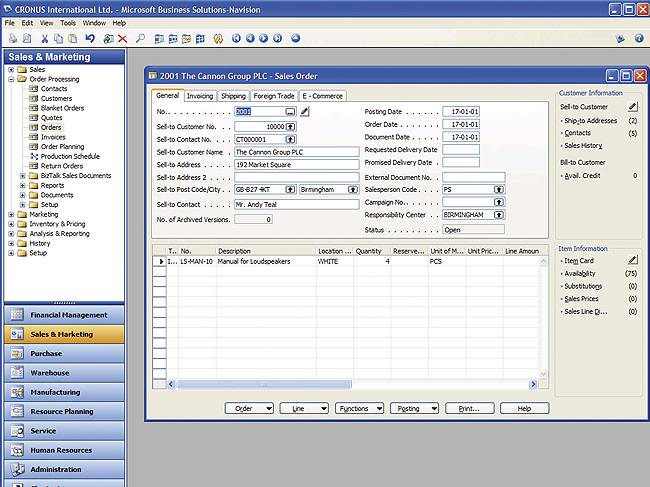
\includegraphics[width=\textwidth]{navision_program.jpg}
%  \caption{Eksempel på Navision program-konfiguration - fra \url{http://www.microsoft.com/business/imagelibrary/businesssolutions/ScreenShotImages/mbs_navision_main_menu_sales.jpg}}alborg kommune har indgået en brugs aftale med Aalborg / Nørresundby Fritidshavn (ANF)
%  \label{fig:navision_program}
%\end{figure}


Et problem med Navision er ifølge Vestre Baadelaug, at man ikke kan lave en regning og sende denne via e-mail \cite{int_vb_sl}. Dette kan dog som tidligere nævnt udbredres ved betaling til supporterende leverandør af Navision.

\subsection{Afgrænsning} % (fold)
Udover kassererens eget system udtalte han sig også om havnefogedens system. Havnefogeden havde ikke noget IT-system til håndtering af pladserne på havnen. Kassereren udtaler \enquote{Havnefogeden holder styr på alle disse informationer på sin egen måde ved en kuvert eller andet} \cite{int_vb_sl}. 

Da det ikke virker til at havnefogeden har et dokumenteret system, aftalte vi et interview med havnefogeden. Interviewet med havnefogeden forløb på samme måde som 3. del af interviewet med Peter Hinrup. Interview blev udført af 3 medlemmer fra gruppen SW2-A405a, med Simon Vandel som referent. Hele interviewet blev optaget på lyd. Alle interviews er transskriberet og vedlagt på cd'en. 

Fokus i problemanalysen vil være på administrationen af bådpladser i en havn. Dette inkluderer både havnefogens arbejdsopgaver, salg af bådlejepladser og medlemmer omkring havnen.
% subsection Afgrænsning (end)
